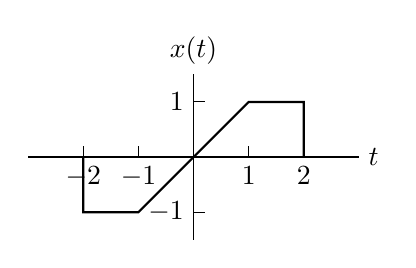
\begin{tikzpicture}[scale=0.70]
	\draw (-3,0) -- (3,0) node[anchor=west] {$t$};
	\draw (0, -1.5) -- (0,1.5) node[anchor=south] {$x(t)$};	
	\foreach \x in {-2, -1, 1, 2}
	{
		\draw (\x, 0.2) -- ++(0, -0.2);
		\node at (\x, 0) [anchor=north ] {$\x$};
	}
	\foreach \y in {-1, 1}
	{
		\draw (0.2, \y) -- ++(-0.2, 0);
		\node at (0, \y) [anchor=east ] {$\y$};
	}	
	
	\draw[thick] (-2, 0) |- (-1, -1)  -- (1,1) -| (2,0);
\end{tikzpicture} 